\documentclass{report}

\usepackage[utf8]{inputenc}
\usepackage[a4paper]{geometry}
\usepackage[myheadings]{fullpage}
\usepackage{fancyhdr}
\usepackage{lastpage}
\usepackage{graphicx, wrapfig, setspace, booktabs, float}
\usepackage{subcaption}
\usepackage[T1]{fontenc}
\usepackage[font=small, labelfont=bf]{caption}
\usepackage{fourier}
\usepackage[protrusion=true, expansion=true]{microtype}
\usepackage{lipsum}
\usepackage{amsmath, amsfonts, amssymb}
\usepackage{mathtools}
\usepackage{fancyvrb}
\usepackage{listings}
\usepackage{textpos}
\usepackage{comment}
\usepackage{afterpage}
\usepackage{array}
\usepackage{makecell}
% \usepackage{pgfgantt}
\usepackage{tikz}
% \usepackage[english]{fancyref}
\usepackage[english]{babel}
\usepackage{color, xcolor} %red, green, blue, yellow, cyan, magenta, black, white
\usepackage{longtable}
\usepackage{tabularx}
\usepackage{multirow}
\usepackage{chngcntr}
\usepackage{subfiles, standalone}
\usepackage[]{algorithm2e}
% \usepackage[skins]{tcolorbox}
\usepackage{rotating} % landscape figures
\usepackage{float}
\usepackage{multicol}
\usepackage{blkarray}
\usepackage{tabularx}
\usepackage{gensymb}
\usepackage{upgreek}
\usepackage{pdflscape, afterpage}
\usepackage{longtable} % For the table in risk assessment
\usepackage[nottoc]{tocbibind}
% \usepackage{breakurl}
\PassOptionsToPackage{hyphens}{url}
\usepackage{hyperref}
\hypersetup{
    breaklinks,
    colorlinks,
    citecolor=black,
    linkcolor=black,
    urlcolor=black
}
\usepackage[natbibapa]{apacite} % needs be loaded after hyperref
% \usepackage[globalcitecopy]{bibunits}
% \defaultbibliographystyle{apacite}
% \defaultbibliography{bibliography}
\usepackage{appendix}
\usepackage{dirtytalk}
\usepackage{syllogism}
\usepackage{soul}
\usepackage{algpseudocode}

\geometry{margin=3cm}

\graphicspath{ {./images/} }

\counterwithin*{equation}{section}
\counterwithin*{equation}{subsection}
\makeatletter
\@addtoreset{equation}{section}
\@addtoreset{equation}{subsection}
\@addtoreset{equation}{subsubsection}
\@addtoreset{equation}{paragraph}
\@addtoreset{equation}{subparagraph}
\providecommand{\leftsquigarrow}{%
  \mathrel{\mathpalette\reflect@squig\relax}%
}
\newcommand{\reflect@squig}[2]{%
  \reflectbox{$\m@th#1\rightsquigarrow$}%
}
\makeatother
\newcommand\tab[1][1cm]{\hspace*{#1}}
\newcommand{\defeq}{\stackrel{\text{def}}{=}}

\definecolor{mygreen}{RGB}{28,172,0}
\definecolor{mylilas}{RGB}{170,55,241}
\lstset{language=python,%
    %basicstyle=\color{red},
    breaklines=true,%
    morekeywords={matlab2tikz},
    keywordstyle=\color{blue},%
    morekeywords=[2]{1}, keywordstyle=[2]{\color{black}},
    identifierstyle=\color{black},%
    stringstyle=\color{mylilas},
    commentstyle=\color{mygreen},%
    showstringspaces=false,%without this there will be a symbol in the places where there is a space
    numbers=left,%
    numberstyle={\tiny \color{black}},% size of the numbers
    numbersep=9pt, % this defines how far the numbers are from the text
    emph=[1]{for,end,break},emphstyle=[1]\color{red}, %some words to emphasise
    %emph=[2]{word1,word2}, emphstyle=[2]{style},    
}

\renewcommand\theadalign{bc}
\renewcommand\theadfont{\bfseries}
\renewcommand\theadgape{\Gape[4pt]}
\renewcommand\cellgape{\Gape[4pt]}

% \newcommand{\HRule}[1]{\rule{\linewidth}{#1}}
\newcommand{\HRule}{\rule{\linewidth}{0.5mm}}
\onehalfspacing
\setcounter{tocdepth}{5}
\setcounter{secnumdepth}{5}


%% Header and footer
% \pagestyle{fancy}
% \fancyhf{}
% \setlength\headheight{15pt}
% \fancyhead[L]{}
% \fancyhead[R]{}
% \fancyfoot[R]{Page \thepage\ of \pageref{LastPage}}

% comment possibilities for all authors
\newcommand{\todo}[1]{\textcolor{green}{TODO: #1}}
\newcommand{\jonas}[1]{\textcolor{purple}{Jonas: #1}}
\newcommand{\julien}[1]{\textcolor{red}{Julien: #1}}
\newcommand{\david}[1]{\textcolor{blue}{David: #1}}
\newcommand{\lukas}[1]{\textcolor{orange}{Lukas: #1}}
\newcommand{\sepideh}[1]{\textcolor{olive}{Sepideh: #1}}

% \date{September 2020}

\thispagestyle{plain} % page numbers!
\pagestyle{plain} % page numbers!


% citations are like: \citep[p.~113]{broome_2012}, \citet[p.~113]{broome_2012}

\begin{document}
\begin{titlepage} % Suppresses displaying the page number on the title page and the subsequent page counts as page
	\center % Centre everything on the page
	\LARGE Maastricht University\\[1.5cm] 
	\Large Research project \\Project report\\[0.5cm]
    \HRule\\[0.35cm]
	{\huge\bfseries Explainable AI: Learning Arguments}\\
	Appendix A\\
	Extended Related Work\\
    \HRule\\[1.5cm]
	\begin{minipage}[t]{0.45\textwidth}
		\begin{flushleft}
			\large
			\textit{Authors}\\Jonas Bei\\ David Pomerenke\\ Lukas Schreiner\\ Sepideh Sharbaf
		\end{flushleft}
	\end{minipage}
	~
	\begin{minipage}[t]{0.45\textwidth}
		\begin{flushright}
			\large
			\textit{Supervisors}\\
			Nico Roos\\ Pieter Collins
		\end{flushright}
	\end{minipage}
	\vfill\vfill\vfill
	{\large\today} % Date, change the \today to a set date if you want to be precise
	\vfill\vfill\vfill % Position the date 3/4 down the remaining page
	%\\[7.5cm]
	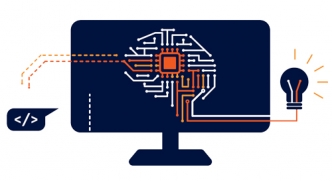
\includegraphics{dke-logo.jpg}\\
	%
\includegraphics[width=0.15\textwidth]{um-logo-250.jpg}
	
	\vfill % Push the date up 1/4 of the remaining page
\end{titlepage}

\begin{abstract}
We investigate \textit{learning arguments}, a family of symbolic machine learning techniques that is particularly human-interpretable. These techniques learn a set of arguments as an intermediate representation. Arguments are small rules with exceptions that can be chained to larger arguments for making predictions. We implement three approaches based on systematic search (naive search, pruned search, and the HeRO algorithm) as well as decision trees and evaluate them on small handmade data as well as medium-sized real world data. We pay special attention to the automatic selection and optimization of a suitable discretization technique, making the approach fruitful for both categorical and continuous data. The results indicate high accuracy for small datasets, yet exponentially increasing computational cost as the dataset increases in size. Learning arguments is highly relevant to the field of explainable artificial intelligence. Our work contributes to widening the spectrum of applications from reasoning tasks in the legal domain to general categorization and prediction tasks.
\end{abstract}

\vfill
{\small\tableofcontents}
\vfill
\newpage

\chapter{Introduction}\label{Introduction}

\section{Explainable AI}

Artificial intelligence, in a societal context, is confronted with a variety of requirements that are recently being investigated by the research fields around explainable, responsible and socially aware artificial intelligence \citep{specialinterestgrouponartificialintelligenceDutchArtificialIntelligence2018}. Here we are concerned with explainability, that is, making the criteria transparent that underlie the decision of an algorithm.

Explainability is also increasingly becoming a \textit{legal} requirement of algorithms. In many countries, which as of recently includes the Netherlands (\citet{raadvanstateECLINLRVS2017} and \citet{rechtbankdenhaagECLINLRBDHA2020}), administrative and judicative decisions that have been supported by an algorithm are required to be comprehensible for judges and citizens \citep{doshi-velezAccountabilityAILaw2019}. The General Data Protection Regulation of the EU (see \citet{goodmanEuropeanUnionRegulations2017}), as well as similar legislation in the United States gives citizens a right to explainabilty also towards companies; albeit only when important decisions such as credit status are involved.

Surveys have been undertaken as to which machine learning techniques are suitable for explainable artificial intelligence, according to a range of sub-criteria. The result is that decision trees and approaches based on deductive logic are the most suitable techniques (\cite{arrietaExplainableArtificialIntelligence2020}; \cite{waltlExplainableArtificialIntelligence2018}). Here we investigate an approach based on argumentation, which can be classified broadly as a deductive logic approach.

\section{Reasoning with arguments}

Giving arguments, considering exceptions to these arguments, and putting multiple small arguments together to build big, convincing arguments, is the human way of justifying things. Automatically learning arguments is relevant for transparent decision making in domains such as law, public administration, or insurance, as well as to the discovery of scientific explanations. 

Argumentation, which will be introduced in \autoref{sec:arguments}, addresses three problems:

The first problem is the mentioned requirement of the explainability of the decision of the algorithm. An algorithm that substantiates its claims with arguments can, if the arguments are properly presented, be understood by a human. Thus, humans can detect potential errors in the algorithm’s decision, or, hopefully, verify that no such errors have been made. This increases trust between human and machine (see \citet{doshi-velezAccountabilityAILaw2019}).

The second problem is that learning from a finite set of data can never lead to generalizations that are completely certain (see \citet{kakasAbductionArgumentationExplainable2020}). This has been studied for centuries as the problem of induction, that is, the problem of deriving laws and law-like generalizations from observations. In the context of machine learning, we can differentiate between the knowledge incorporated in the set of training data and the background knowledge of human experts. Today, there is usually some relevant knowledge that only experts (or even non-expert humans) possess, which is not incorporated in the training data set. Such knowledge could be about the causal relationships between some of the attributes of the data, for example. Machine learning systems that produce arguments can leverage the knowledge of both the data set and the human: The system can generate a handful of arguments of arguments for (and potentially also against) a decision, and the human can then decide which of these make sense, and which are most credible.

The third problem is that humans may pose certain requirements towards the justification of a decision that are in conflict with the training data. An important example is racial, sexual, and other bias, that may be present in the training data, and would lead to the perpetuation of discrimination (and hence, further biased data sets) in the future. In order to avoid vicious circles of discrimination, humans may wish to reject discriminatory decisions, even if they are justified given the training data. This may also be realized with argumentation, where, for example, racially motivated arguments can be discarded and the most plausible of the remaining arguments can be used.

\section{Research questions}

\begin{enumerate}
    \item Can we reproduce the examples from \cite{verheijProofProbabilities2017} and \cite{verheijAnalyzingSimonshavenCase2020}?
    \item Can we find an (efficient) algorithm for learning arguments with this approach? How do we decide which arguments are relevant and which ones can be discarded?
    \item Can we transfer the approach to a general attribute-value classification machine learning setting?
    \item What existing techniques are there for learning arguments, and how do they relate to each other? What insights can we transfer to the implementation of the approach by \cite{verheijProofProbabilities2017}?
    \item Can we show the (in)applicability of the approach on a real dataset? How does the approach compare with similar rule-based approaches in terms of (a) accuracy and (b) runtime on %(1) 
    real world data sets 
    % and (2) tailored synthetic data sets
    ?
    What can we infer about explainability by looking at the theories generated by the algorithms?
\end{enumerate}

\label{theory}
\chapter{Theory}

Here we present and critically investigate \textit{proof with and without probabilities}. \citet{verheijProofProbabilities2017} formally defines the notion of a \textit{case model} and three different notions of arguments.

\section{Case models}

\begin{figure}[htb]
        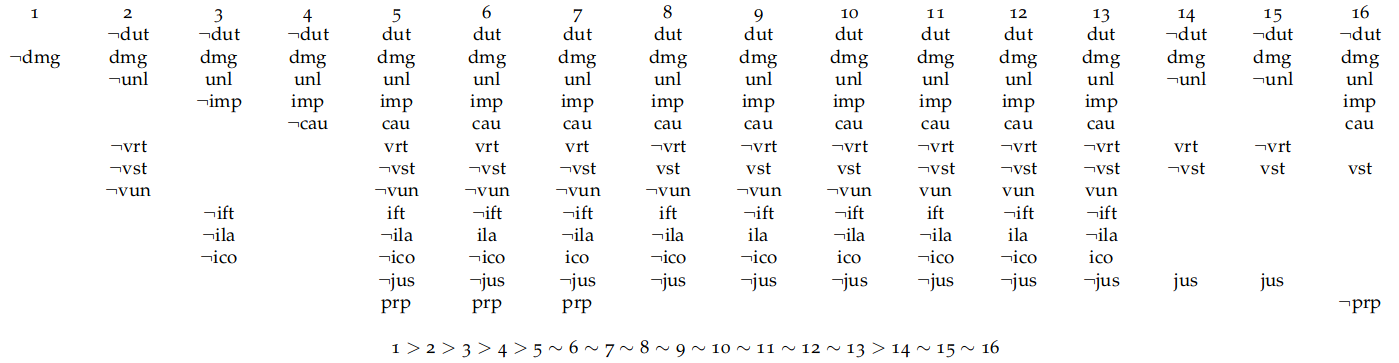
\includegraphics[width=\textwidth]{images/casemodel.png}
        \caption{Case model for Dutch law of unlawful acts. From \citet[fig.~23]{verheijArgumentsGoodArtificial2018}.}
        \label{fig:casemodel}
\end{figure}

A case model is a set of weakly ordered \textit{cases}, where each case is distinguished by the propositions that follow from it. We can alternatively define a case as the most general proposition which entails the propositions that follow from the case. 

For our purposes, we can restrict the definition of a case by demanding that it consists of a conjunction of literals. Then, we deal with cases that contain disjunctions of propositions by splitting them into multiple cases. This way, we arrive at a boolean (propositional) representation that is suitable for machine learning. We do this by interpreting a scenario as a data point in the training data.

One challenge is how to derive the preference relation over cases from the training data. The preference relation is relevant for identifying presumptively valid arguments. One approach here is the following: When we test whether an argument with a specific set of literals in the conclusion is presumptively valid, we aggregate the training data by the set of attributes that corresponds to the set of literals in the conclusion. We then take the count how many cases have been aggregated into one single case as an indication of how preferred this case is. 

\label{sec:arguments}
\section{Arguments}

\begin{figure}[htb]
        \centering
        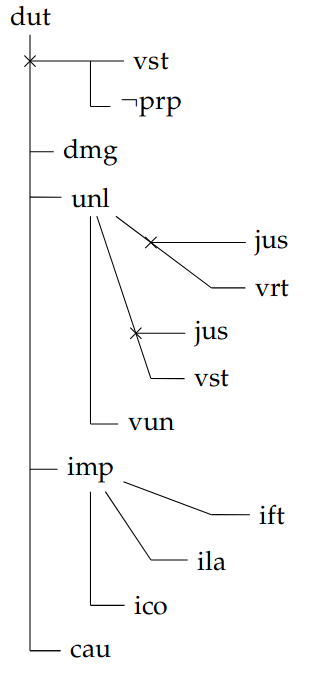
\includegraphics[width=0.15\textwidth]{images/argument.png}
        \caption{Argument structure (right) for Dutch law of unlawful acts. From \citet[fig.~5]{verheijArgumentsGoodArtificial2018}.}
        \label{fig:argument}
\end{figure}

In the context of this research project, the notions of conclusive and of presumptively valid arguments are interesting. The notion of a coherent argument is only interesting in so far as it is a condition for the two other types of arguments. 

\subsection*{Conclusive arguments}
An argument is \textit{conclusive} according to \citet{verheijProofProbabilities2017} if the conclusion is true in every case where the premises are true.

This raises the question whether an argument that is \textit{conclusive} in the sense of \citet{verheijProofProbabilities2017} is also conclusive in the sense of everyday language. There is no formal requirement on case models that they need to be exhaustive. Thus, we can imagine that in the real world (though not in the case model) the premises of an argument may hold and the conclusions may simultaneously not hold, but it would still be \textit{conclusive}  in the sense of \cite{verheijProofProbabilities2017}, just because this real world case is not included in the case model. Hence, the notion of an argument being \textit{conclusive} is misleading to a certain extent. We can fix this by adding the assumption that the case model exhaustively represents all the cases that hold in the real world; this may well be an implicit assumption of the original approach. 

When applying the approach to machine learning, the problem is anyway that the training data will normally never contain exhaustive data, and the idea of deriving conclusive arguments is vain -- consider the problem of induction. To get a probabilistic idea, we can utilize the idea of \textit{Bayesian smoothing}, which is epistemologically quite attractive. Bayesian smoothing in its standard variant of \textit{1-smoothing} states that the probability of an event that occurs $k$ times in a data set of size $n$ is not $\frac{k}{n}$, but rather $\frac{k}{n+1}$. (This is for binary data without prior probabilities only, and can be adjusted otherwise towards \textit{k-smoothing} or similar.) A \textit{conclusive} argument in the sense of the definition, then, is only valid probabilistically, resembling a strong presumptively valid argument.

\subsection*{Presumptively valid arguments}

An argument is \textit{(presumptively) valid} if the conclusion is true in the most likely or most preferred case in which the premises hold. Presumptively valid arguments are most interesting in the context of this project, since (a) they can have exceptions and are thus very much like human arguments, which is desirable from an explainable AI perspective, and (b) due to the strong conditions there will usually be only very few conclusive arguments in real world data, and the bulk of the arguments will be presumptively valid only. 
\label{related_work}
\chapter{Related work}
 
Here we give a concise overview over the most relevant related work. A more detailed survey can be found in \autoref{appendix-related-work}.

\section{Argumentation}

Arguments are defeasible rules or chains of such rules that explain decisions, such as predictions and categorizations. We can find examples of such explanations in our daily lives, and, in a more formal setting, in legal decisions and medical diagnoses.

Argumentation has been formalized by \cite{dungAcceptabilityArgumentsIts1995} and implemented in \textit{ASPIC+} \citep{modgilASPICFrameworkStructured2014}. \cite{roosResolvingConflictsArguments2000} formalizes argumentation in the context of logic. Arguments can be built from a \textit{defeasible theory}, consisting of facts, strict rules, and defeasible rules. The defeasible rules are partially ordered by a preference relation, such that in the case of conflicting rules, the conflict can be resolved by ignoring the less preferred rule. The preference relation can be derived by ordering the defeasible rules according to their specificity. Reasoning with defeasible theories is possible by using an argumentation tableau \citep{roosSemanticTableauMethod2020}. An overview over implementations of argumentation is provided by the \textit{Tweety Project} \cite{thimmTweetyProjectComprehensiveCollection2021}.

\section{Learning arguments}

The learning of rules or arguments can be regarded as either a supervised or unsupervised learning task. Framing the task as unsupervised puts emphasis on the quality of the arguments themselves; framing it as supervised puts emphasis on the quality of the predictions. 
% Here we are mostly concerned with the quality of the rules themselves, rather than with their predictive accuracy, so the task is best framed as unsupervised. 
The representation of both data and hypotheses is a relational representation in the original approach in \cite{verheijProofProbabilities2017}, restricted to propositional logic. In this project we investigate transfering the approach to work on input data with an attribute-value representation. (On machine learning representations, see \cite{deraedtLogicalRelationalLearning2008}.)

\cite{kakasAbductionArgumentationExplainable2020} give an insightful overview over argumentation in machine learning, enumerating multiple use cases of arguments. Here we are concerned with argumentation as the target language for learning. Within this use case, they distinguish two paradigms. In the first paradigm, arguments are potentially large monolithic rules that directly map input facts to output facts. This paradigm comprises decision lists, exception lists, inductive logic programming with exceptions, and random forest methods. In the second paradigm, arguments consist of multiple chained smaller arguments, with intermediate concepts connecting the arguments. The smaller arguments describe local relations, that is, relations that only involve a small number of attributes. Within this paradigm fall the \textit{NERD} algorithm \citep{michaelCognitiveReasoningLearning2016}, \textit{machine coaching}, and \textit{SLAP}.

Two algorithms are explicitly concerned with the mining of defeasible rules: Firstly, the \textit{DefGen} algorithm uses association rule mining, for which highly optimized algorithms for big data exist, and postprocesses the output by applying relevance criteria \citep{governatoriApplicationAssociationRules2001}. This high-level structure can also be found in our \textit{pruned search} algorithm introduced in \autoref{sec:pruned-search-meth}, but the pruned search algorithm has been developed independently from DefGen. Secondly, the \textit{HeRO} algorithm iteratively applies the criterion of \textit{information gain}, taking inspiration from decision list mining and covering rule algorithms. We have implemented the HeRO algorithm and give an overview over it in \autoref{hero-meth}.

\section{Other rule-based learning approaches}

Competing approaches for the explainable learning of rules are decision trees, relational learning and inductive logic programming, and probabilistic and causal networks.

While decision trees are equivalent to sets of classification rules (\cite{wittenDataMiningPractical2017}[ch. 3.4], \cite{hanDataMiningConcepts2011}[p. 358]), the rules to which they correspond are long and unstructured; domain experts prefer to work with well-structured sets of arguments, which then can be easily transformed into decision trees for classification \citep{breidenbachTextCode2021}. The advantage of decision trees is their suitability for big data. Some of the mentioned disadvantages can be overcome by pruning the decision tree (see also \autoref{dectrees-meth}).

Relational learning and inductive logic programming are concerned with the learning of first-order logic and logic program representations, respectively, which can potentially be downgraded to work on propositional logic or attribute-value representations \citep{deraedtLogicalRelationalLearning2008}. Usually, algorithms in these fields produce monotonic rules. These do also allow for the construction of arguments, but these arguments cannot defeat each other and are therefore less similar to everyday argumentation than arguments from nonmonotonic rules. One possibility for simulating exceptions is to use an exception predicate for each rule that has an exception. \cite{dimopoulosLearningNonmonotonicLogic1995} explore the theory of nonmonotonic logic programming, \textit{XHAIL} \citep{rayInferringProcessModels2007} and \textit{TAL} \citep{corapiInductiveLogicProgramming2010} provide algorithms.

Probabilistic networks are most suitable for reasoning with uncertainty. Causal networks present an improvement over probabilistic networks (and all other methods) by taking into account the causal relationships between the variables. Machine learning methods usually assume that future examples are drawn from the same fixed probability distribution as past examples \citep{russellArtificialIntelligenceModern2010}[p. 708, 714]. Causal networks, in contrast, allow for counterfactual reasoning \citep{russellArtificialIntelligenceModern2020}[ch. 13.5.2]; moreover, experiments indicate that it is easier to reason causally than it is to reason diagnostically \citep{kahnemanJudgmentUncertaintyHeuristics1982}[p.121-128]. Ranking theory \citep{spohnLawsBeliefRanking2012} replaces probabilities with a preference relation representing disbelief in probabilistic and causal networks, providing a potential
unexplored connection to argumentation.

\section{Propositionalization}

In this project, we aim to transfer a learning method that works on discrete propositional input data to work on attribute-value input data, including categorical and continuous attributes. Our approach here is to preprocess the input data by transforming continuous and categorical attributes into propositions. Some techniques for propositionalization are described in \cite{deraedtLogicalRelationalLearning2008}. The propositionalization techniques explored in this project are Equal-Width Binning, Equal-Depth Binning, K-Means and DBSCAN, where each of the algorithms has its respective strengths and weaknesses. Equal-Width Binning and Equal-Depth Binning are the approaches with the least complexity, and K-Means and DBSCAN are more complex.

\chapter{Techniques used}\label{Methodology}

In this section, the process of learning arguments is discussed in its entirety.

\section{Discretization Techniques}\label{Section_Discretization_Techniques}

With the exception of decision trees, the rule-mining algorithms in this project cannot be trained on continuous data. Therefore, in order to apply the rule-mining algorithms to datasets, we must rely on data discretization techniques to preprocess the data before mining the rules. In the data, every numerical feature of a dataset is considered to be continuous.

\subsection*{Equal-Width Binning}
This algorithm is a comparatively simple binning technique. Here, the range spanned by the smallest and largest value of a feature (referred to as $min$ and $max$ respectively,) is divided into a number of bins $k$, where each of these bins have size $\frac{max-min}{k}$. To discretize, values are assigned to the respective bin they fall into.

% JONAS: "Instead of talking about general flaws of the algorithm, we will focus on the performance of the algorithm in our experiments."

% This approach is easy to implement and not computationally expensive. However, there are some notable flaws: This algorithm assumes that each cluster has the same diameter, and it is prone to outliers due to reliance on minimum and maximum values of a feature. 

\subsection*{Equal-Depth Binning}
Equal-depth or equal-frequency binning is another simple discretization approach. Here, values are assigned to one of $k$ bins, such that each bin approximately holds the same number of instances. This is done by sorting the values of the feature and assigning $\frac{n}{k}$ of the sorted instances into each bin, where $n$ is the number of total values.

\subsection*{Clustering approaches}

To discretize more complex features in the data, clustering approaches are considered. Here, values of a given feature in the data are clustered, and replaced by the discretized value. In the dataset, clusters are represented as ranges, where each cluster is described by its smallest and largest value. By the nature of the given clustering algorithms, these ranges do not overlap.

\subsubsection*{K-Means Clustering}
K-Means \citep{LeastSquareLloyd} is based on the idea of centroids, which are points in the centre of the cluster. Here, $k$ centroids are initialized randomly, and the instances are assigned to the cluster whose centroid is closest. Then, the centroids are moved to the mean of the cluster, and the instances are assigned to their new cluster. The algorithm converges when the movement of centroids is below a certain threshold.

% One flaw of this algorithm is that it is sensitive to outliers due to reliance of mean values. It is also highly dependant on the random initialization. Additionally, this algorithm assumes that every cluster has a similar diameter, which may not be true for some datasets.

\subsubsection*{DBSCAN Clustering}

DBSCAN  by \citet{DBSCANPaper} considers clusters to be regions of high density. For each instance, the algorithm counts the number of instances within a distance $\epsilon$, also called the instance's $\epsilon$-neighbourhood. If this number of neighbours of an instance surpasses a given threshold, the instance is considered to be a core instance, an instance within a dense region. The neighbours of this core instance are considered to be in the same cluster, where some neighbours may also be core instances themselves. Therefore, a cluster consists of a multitude of core instances. 
% This algorithm can fail in identifying clusters if density varies for clusters, or for spare regions of a feature.

\subsection*{Cluster Optimization}

The aforementioned clustering algorithms all provide parameters that can be tuned in order to find  clusters representing the data correctly. In this project, the silhouette score introduced by \citet{ROUSSEEUW198753} has been utilized to provide a metric for accuracy of clusters. This score computes the mean silhouette coefficient of all samples (given by equation \ref{Silhouette_Coefficient}).

\begin{equation}
\label{Silhouette_Coefficient}
    silhouette\_ score = \frac{b - a}{\max(a, b)}
\end{equation}

\noindent In equation \ref{Silhouette_Coefficient}, $a$ denotes the mean distance to the other instances in the same cluster (intra-cluster distance) and $b$ denotes the minimal distance to another instance that is not part of the same cluster (nearest-cluster distance).

Clusters are optimized by exhaustive search this project, i.e., every combination of parameters is tested using the silhouette score, before returning the parameters resulting in the highest score.

\subsection*{Discretization of prediction data}

Once the data is discretized and rule-mining is performed, rules have to be applicable to the original, continuous features in order to predict the outcome. While discretized values are represented as ranges of the minimum and maximum value of the given bin or cluster, not all values to be predicted may fall into these given bins. Therefore, to discretize the new values, distances are measured to each of the boundaries of a given bin. Then, the value is assigned to the bin with the smallest distance for either boundary.

\section{Learning arguments}\label{Section_Learning_Arguments}

% Skip this for proofreading for now, will rewrite most of it

We have implemented four different algorithms for learning arguments from data. The first two algorithms are devised by ourselves, the third one is implemented by ourselves according to the high-level description in \cite{johnstonInductionDefeasibleLogic2003}, and the fourth one is based on the open-source library \textit{scikit-learn} \citep{pedregosa2011scikit}.

\subsection{Naive search}

The naive search algorithm follows the generate-and-test paradigm: Firstly, all possible arguments are generated, and secondly they are tested whether they are conclusive, presumptively valid, or coherent. The generation of all possible arguments is very inefficient: For a dataset with $k$ columns and $n$ bins per column, the space of all sensible combinations of literals is of size $n^k$. The algorithm is therefore only suitable for very small datasets such as the toy examples in \autoref{appendix-notebook}.

An important feature of the naive search is the postprocessing of the rules, consisting of (1.) filtering and (2.) merging:

\begin{enumerate}
    \item The filtering step is necessary for removing irrelevant rules. For example, when there are two arguments $a \rightsquigarrow d$ and $a \land b \land c \rightsquigarrow d$, then the second argument is more specific than the first argument and therefore only relevant if there is another relevant argument, such as $a \land b \rightsquigarrow \neg c$, to which it is an exception. Generally speaking, an argument A is relevant if there is no less specific argument to A, or if A is an exception to a relevant argument. We say that an argument $(P_1, c_1)$ is more specific than another argument $(P_2, c_2)$, if its premises $P_1$ are a proper superset of the premises $P_2$ of the other argument. 
    \item During the argument generation, we only generate arguments with a conclusion of a single literal. We reduce the number of arguments for legibility by merging together any arguments $(P_1, c_1)$, ..., ($P_m, c_m)$ that have the same premises $P_1=...=P_m$ to a single argument $(P_1= ...= P_2, \{c_1\} \cup ... \cup \{c_m\})$ with multiple conclusions.
\end{enumerate}

\label{sec:pruned-search-meth}
\subsection{Pruned search}

\begin{figure}[htb]
        \centering
        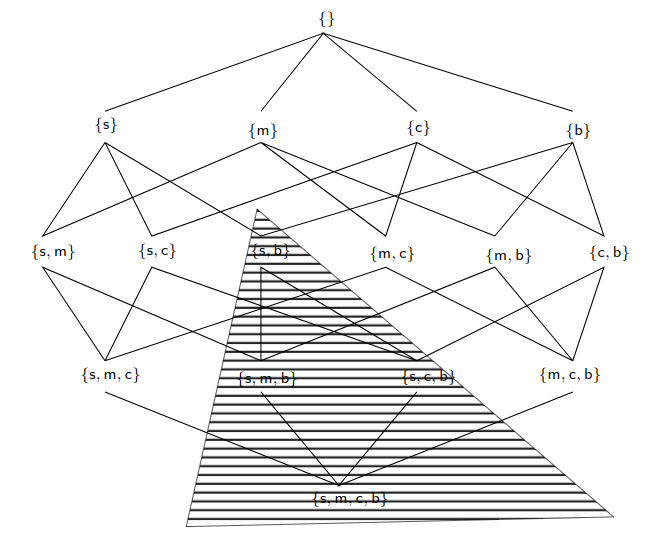
\includegraphics[width=0.6\textwidth]{images/pruning.png}
        \caption{\textit{Pruning specializations.} From \citet[p.~52]{deraedtLogicalRelationalLearning2008}. All $2^n$ subsets of $\{s, m, c, b\}$ are systematically searched, starting from the most general set at the top. Knowing that the set $\{s, b\}$ is infrequent allows us to prune all its specializations, which is a lot. }
        \label{fig:pruning}
\end{figure}

\label{pruned-search}
\begin{algorithm}
\caption{Pruned search.}
\For{each literal p}{
    search(premises=$\varnothing$, target=p, depth, max\_size)\\
    remove arguments that are more specific to another argument \\
    \hspace{1cm}but are no exception to another argument\\
    merge arguments with the same premises
}
$\vspace{0.5cm}$
\Function{search}{premises, target, depth, max\_size}: \\
candidate\_arguments := $\{(\text{premises} \cup \{p\}, \text{target}) | p \in \text{literals}\}$ \\
determine and save which candidate arguments are \\
\hspace{1cm}conclusive, presumptively valid, and coherent given the data \\
\For{each presumptively valid argument (P, c)}{
    search for exceptions: \\
    \For{each literal p about the same fact as c, except c itself}{
        \If{depth $> 0$}{
            search(premises=P, target=p, depth - 1, max\_size)\\
            save the results
        }
    }
}
\For{each $(P_1, P_2), \text{where}\\
    \hspace{2.5cm} (P_1, c_1) \in \text{candidate\_arguments}, \\
    \hspace{2.5cm} (P_2, c_2) \in \text{candidate\_arguments}, \\
    \hspace{2.5cm} |P_1 \cap P_2| = |\text{premises}|,\\
    \hspace{2.5cm}|\text{premises}| < \text{max\_size}$ \\
}{
    search for more specific arguments: \\
    search(premises=$P_1 \cup P_2$, target=target, depth, max\_size) \\
    save the results
}
\EndFunction
\end{algorithm}

\noindent The pruned search algorithm improves the runtime by pruning the search space in a systematic way. This technique is known from frequent pattern mining (and its application to association rule mining; see \cite{agrawalFastAlgorithmsMining1994}), and is described in the context of logical learning in \cite{deraedtLogicalRelationalLearning2008}. The idea is to identify a quality criterion, for which the following is true: If a set fulfils the quality criterion, all its subsets must also fulfil the quality criterion. (Alternatively: If a set fulfils the quality criterion, all its \textit{super}sets must also fulfil the quality criterion; this an be visualized by "flipping" the search space or the direction of the search). For example, in the context of frequent pattern mining, if a set is frequent, then all its subsets must also be frequent. The principle of pruning the search space is visualized in \autoref{fig:pruning}.

This raises the issue of the selection of a suitable quality criterion for pruning the search space in our application of learning arguments. We find two quality criteria: 

\begin{enumerate}
    \item \textit{If an argument $(P, c)$ is conclusive, then all coherent arguments $(P', c)$ must also be conclusive, for all $P'$ that are a superset of $P$.} 
    % (Proof: The argument $(P, c)$ is conclusive iff $c$ holds in all cases where $P$ holds. ...
    % However, the arguments $(P', c)$ need not be coherent, and thus in an additional step the coherence ... not sure!
    \item \textit{If an argument $(P, c)$ is coherent, then all arguments $(P', c)$ must also be coherent, for all $P'$ that are a subset of $P$.}
\end{enumerate}

The most important part of the learning algorithm in terms of efficiency is the learning of presumptively valid argument: They are relevant for a prediction, and there are equally many or (usually) many more  presumptively valid arguments than conclusive arguments. So it would be nice if we could find a quality criterion for learning presumptively valid arguments. Unfortunately, presumptive validity, unlike conclusivity or coherence, is not itself a quality criterion: 

\textit{Proof by contradiction:} Consider the case model $ (1, \{a,b,c,d\})\}, (2, \{a, b, \neg c, \neg d\}), \{(3, \{a, \neg b, \neg c, d\})$. A higher number denotes a higher priority of the case. $(\{a, b\}, \neg d)$ is a presumptively valid argument in the case model, since the case with the highest priority where its premises hold is the second case; and its conclusion also holds in the second case. \\
Assume that presumptive validity is a quality criterion. So, either (a) if an argument $(P, c)$ is presumptively valid, then all arguments $(P', c)$ must also be presumptively valid, for all $P'$ that are a subset of $P$; or (b) if an argument $(P, c)$ is presumptively valid, then all arguments $(P', c)$ must also be presumptively valid, for all $P'$ that are a superset of $P$. Consider (a): Then $(\{a\}, \neg d)$ must also be presumptively valid. But the most likely case where the premises hold is the third case, and there its conclusion does not hold, so it is not presumptively valid, contradiction. Consider (b): Then $(\{a, b, c\}, \neg d)$ must also be presumptively valid, but the most likely case where its premises hold is the first case, and its conclusion does not hold there, so it is not presumptively valid, contradiction. Contradiction in (a) and (b), and either (a) or (b), so overall contradiction.\\
Thus, presumptive validity is not a quality criterion, no matter in what direction we would like to prune the search space.\square

We cannot use presumptive validity itself as a quality criterion for pruning the search space, but we can at least use a condition for presumptive validity: Coherence. \autoref{pruned-search} shows our algorithm, which uses coherence to prune the search space. We separately start a search for each literal (each combination of column and bin), looking for arguments with this literal as a conclusion. After search is completed, we filter and merge the resulting arguments in the same way as described for the naive search algorithm. At each search step $i$ we consider arguments with $i$ premises (that is, a premise size of $i$). 

At the end of the search step we gather all coherent arguments of the step, and check all combinations of these arguments whether their premises are different in exactly two literals. The reason is: If they are different in two literals, we can take the union of the premises as a new premise of size $i+1$, and we know that many subsets of this premise lead to a coherent argument. Consider, for example, two premises $\{a,b,c,d\}$ and $\{b,c,d,e\}$: The union is $\{a,b,c,d,e\}$ with size $n=5$. Enumeration shows that $2^n-2^{n-2} = 24$ of its subsets are also subsets of at least one of the two premises of which we already know that they are coherent. It is thus much more likely for the new premise to also be coherent than it would be for an arbitrary premise. 

This principle of combining small sets fulfilling the quality criterion into larger sets likely to fulfil the quality criterion is known from the Apriori algorithm (see \cite{tanIntroductionDataMining2014}). There, it makes the algorithm suitable for big datasets. Here, because coherence is only a condition but not the same as presumptive validity (which we are looking for), it at least makes the algorithm efficient enough for the medium-sized datasets we use.

\label{hero-meth}
\subsection{HeRO algorithm}
% HeRO algorithm is a kind of method for computing square roots 

\begin{figure}[htb]
        \centering
        
\includegraphics[width=0.4\textwidth]{images/hero.jpg}
        \caption{\textit{Hero algorithm.} \textcopyright Curvabezier, dreamstime.com}
        \label{fig:hero}
\end{figure}

The HeRO algorithm has been devised by \cite{johnstonAlgorithmInductionDefeasible2003}, and the research behind it, like \cite{verheijProofProbabilities2017}, is also originally targeted towards the legal domain \citep{johnstonInductionDefeasibleLogic2003}. It does not primarily perform a systematic search, but rather an incremental search: At each step, it considers which argument would be most valuable to be added to the theory in order to increase the accuracy the most; and then it adds the most valuable argument to the theory and asks the question again, until there is no more argument that can increase the accuracy. 

The algorithm builds up a totally ordered set of arguments, and at every step it considers all positions (before, after, or between the existing arguments) for adding the next argument. For determining the most valuable argument (and its most valuable position), the criterion of \textit{information gain}, that is increase in accuracy on the training set, is used. Similar to the pruned search algorithm presented above, the HeRO algorithm also starts by considering simple arguments and then in some cases also considers arguments where the premises are more specific. The mechanism for deciding whether more specific premises should also be considered uses the criterion of \textit{maximum information gain}. The maximum information gain of an argument is the highest information gain that can be achieved by any argument that is more specific. This is equivalent to the information gain that would be achieved by adding an argument that correctly predicted all the rows where the premises hold. 

Formulas for information gain and maximum information gain and a high-level pseudocode algorithm are provided in \cite{johnstonAlgorithmInductionDefeasible2003}. The authors also briefly mention a few optimization techniques, which we have not implemented. There is no public implementation of the HeRO algorithm, so we are the first to provide a such. Since the description by the authors is on a high level only, our algorithm, apart from the optimizations, may also differ from the original algorithm in other minor ways. 

\label{dectrees-meth}
\subsection{Decision trees}

To classify by building tree models, the open-source library \textit{scikit-learn} \citep{pedregosa2011scikit} is used. This implementation utilizes the CART \citep{DecTreePaper} algorithm. Here, the tree is built choosing a feature $k$ and a threshold $t_k$ by using a cost function measuring the purity of the subsets produced by the split. In this project, this is measured by the Gini impurity introduced by \citet{DecTreePaper}. Once the split has been made, the algorithm iteratively splits the subsets further, until a given maximum depth is reached, or no split reducing impurity can be found.

In a decision tree, the nodes at the bottom of the tree are referred to as leaf nodes, or internal nodes. Trees can be converted into decision rules, where each leaf node is associated with one rule. Here, the path traversed through the decision tree represents the premises that must hold for the conclusion at the child node.

\subsubsection*{Hyperparameter Tuning of Decision Trees}\label{Section_Bayesian_Optimization}

To maximize performance of the decision tree algorithm, various hyperparameters can be tuned. In this project, this is done via Bayesian Optimization \citep{BayesOptPaper} utilizing the \textit{scikit-optimize} package \citep{skopt}. This algorithm samples points to construct an interpolation function, also called posterior function. This function represents the objective function (which, in this case, is a function measuring the accuracy of the tree with its parameters as inputs). New points are found using an acquisition function, which balances exploration and exploitation by calculating uncertainty in the posterior function. These query points are then used to update the posterior function. After a given number of iterations, the algorithm converges, returning an estimate of the optimal parameters by using the posterior function.
\chapter{Experimental results}

In order to test the performance of the algorithm, several experiments have been performed.

\section{Set-up}
In order to evaluate the framework described above, a wide variety of experiments is conducted in order to gain some insight which rule mining technique, as well as discretization method, lead to a high predictive power. In some cases the algorithms require additional hyperparameters which are included in the analysis as well. 

The four main steps of the experiments are data preprocessing, model training, predictions, as well as model evaluation. In a first step, the data is discretized by a method described in section \ref{Section_Discretization_Techniques}. For one experiment using decision trees, only the target column is discretized. In a second step, the selected algorithm (see section \ref{Section_Learning_Arguments}) for learning the arguments from the data is applied. Afterwards, the learned model is used to generate predictions from the in-sample as well as out-of-sample data. Finally, the predictions are evaluated by computing accuracy and weighted F1-score. Despite being hardware dependent, the training time is measured in order to get an understanding of the relative computational cost of the algorithms. 

\paragraph*{Discretizing the data}
The data is discretized using equal-width binning, equal-depth binning, DBSCAN and k-means. The parameter to be defined in this step is mainly the number of bins that the data will be discretized into. An optimization algorithm for finding the ideal number of bins has been implemented. However, due to the fact that the search algorithms are very sensitive to the number of bins, the discretization algorithms also run with some predefined number of bins, namely two, three and four bins. 

\paragraph*{Learning Arguments}
While the decision tree algorithm optimizes the parameters by Bayesian Optimization (section \ref{Section_Bayesian_Optimization}), there is still a need for specifying the parameter search space. Here, the maximum features randomly chosen at a split can be between 1 and the number of features of the training data. The maximum depth is capped at 50 to retain explainability and the minimum number of samples required at a leaf node is constrained between 1 and 1000. The minimum number of samples required to split an internal node is between 2 and 1000. 
 
For the pruned search algorithm, there are mainly two hyperparameters that need to be tuned. Next to the search depth, which is tested with the values {1, 5, 20, 50}, the values {2, 4, 6} are tested for the maximum premise size constraint. A priori, we assume that the former will have a significant impact on the run-time while the latter will mainly determine the the quality of the predictions. 

Lastly, the hero algorithm does not require any hyperparameter tuning. 
 
\section{Results}

\paragraph*{Decision Trees} When using the Boston Housing Data set, the decision trees were scoring a perfect accuracy of 1 when using equal-depth binning or equal-width binning. Using DBSCAN gave a slightly lower accuracy of 0.99 and using k-means yielded 0.86. Those figures showcase very well the impact and importance of choosing a good technique when discretizing the data. Note that the accuracy alone does not provide a complete picture of the quality of the algorithm: For example, using one bin for all the data would result in a accuracy of 1, yet the algorithm would not explain any structure in the data. With regard to the training time, the decision trees run significantly longer than the pruned search algorithms. When only discretizing the target column using equal-width binning and leaving the input values continuous, the decision trees achieve an accuracy of 0.92. This indicates that the decision trees are able to capture the structure well. 

\paragraph*{Pruned search} When it comes to pruned search, the results also exhibit high results for the accuracy and F1 scores. The average accuracy (F1 score) on the training set is 0.88 (0.83) and 0.85 (0.83) on the test set. In total, 198 experiments with the pruned search algorithm have been run and the standard deviation of the evaluation metrics (accuracy: 0.0868, F1: 0.0864) indicate that the algorithms performance is rather robust. When studying the correlation, one notices that the pruned search algorithms do not significantly vary in precision when adjusting search depth and maximum premises. Table \ref{tab:pruned search} shows the correlation of the hyperparameters as well as the precision. In this case, runs on the test set and training set are considered together. Contrary to the initial hypothesis, a constraint on premises does not have an effect on the performance, yet a positive correlation to the run-time suggests that it increases the computational complexity significantly. The number of bins are positively correlated with the run-time, yet exhibit a negative correlation on the accuracy metrics. Since fewer bins make the problem easier for the algorithm, this does not come as a surprise. A very interesting observation is the negative correlation of the the run-time and precision. This indicates that simpler and faster algorithms perform better on this data set, likely because they are less predisposed to overfitting. 

As mentioned, the discretization algorithm has a siginificant impact on the success of the algorithm. When looking at the situation where pruned search is used to mine the arguments and the number of bins is fixed to 2, one can observe that the accurancy on the test set increases when using the discretization algorithms in the following order: k-means (average accuracy 0.80), equal depth binning (0.83), equal width binning (0.91), DBSCAN (0.97). The ordering is strict, meaning that using a different discretization algorithm will always yield a higher or lower accurancy in the given settings. This emphasizes the  significant impact of binning on the algorithm's performance. 

\paragraph*{HeRO} The HeRO algorithm behaves similar compared to the pruned search algorithm in terms of performance. Similar as outlined above, the discretization algorithm is the main driver for the algorithm's performance. While the equal-depth binning yields an average accuracy (F1) of only 0.53 over all experiments, using k-means improves the results already significantly with an average accuracy of 0.79 (0.70). Equal-width binning further improves the situation by yielding 0.91 (0.86) and with an average accurancy 0.95 (0.93), DBSCAN gives the best results for the HeRO algorithm.


\begin{table}[h]
\centering
\begin{tabular}{lllllll}
\multicolumn{1}{c}{\textit{n=198}} & \textit{Acc} & \textit{F1} & \textit{No. bins} & \textit{Depth} & \textit{Runtime} & Max premises                                    \\ \hline
Acc                                                                               & 1.000        &             &                   &                &                  &                                                 \\
F1                                                                                & 0.940        & 1.000       &                   &                &                  &                                                 \\
No. bins                                                                          & -0.008       & 0.057       & 1.000             &                &                  &                                                 \\
Depth                                                                             & 0.000        & 0.000       & 0.000             & 1.000          &                  &                                                 \\
Runtime                                                                           & -0.173       & -0.001      & 0.170             & 0.035          & 1.000            &                                                  \\
Max premises                                                                      & 0.000        & 0.000       &                   &                & 0.207            & 1.000                                           \\ \hline
\end{tabular}
\caption{Pruned Search Hyperparameter Correlation Table}
\label{tab:pruned search}
\end{table}

\section{Discussion}

The experiments show that the approach is generally working, yet needs further efforts to become practically applicable. There are two main issues that the experimental results bring to light. The first one is the exponentially increasing computational complexity of both the search and discretization algorithms. In this case, the amount of columns of the dataset has been reduced, and the Boston Housing data set only has about 500 data points. However, discretizing and training the algorithm in this setting already takes quite some time on end user hardware. These limitations should likely be  addressed first.

Another point worth mentioning is the binning itself. In cases where the data is binned in very few bins, it can happen that the data is heavily skewed due to outliers. When e.g. 95\% of the houses are categorized as 'high price', the algorithm will score a very high accuracy with a naive prediction of always predicting 'high price'. It is obvious that the ability of the algorithms to explain patterns in data will decrease if the number of bins is reduced, while accuracy tends to increase. For that reason, just considering the accuracy might lead to false conclusions. 

Furthermore, the experiments showed that simpler algorithms with less shorter seem to do better than the more complex algorithms. The key takeaway from this may be that learning arguments tends to over-fit quickly. Especially when the learned arguments have a lot of premises, one would need to learn a lot arguments in order to find a prediction for unseen data. Particularly when the test data has a different distribution that the training data, it might become rather challenging for the algorithms to generalize well. 


\section{Qualitative analysis}

In the following, we inspect in some more depth the theories that the different algorithms learn on small toy examples. More such comparative examples can be found in \autoref{appendix-notebook}. We do not include the decision tree algorithm in this section because we have not implemented it to learn from case models, but only from formatted data sets; in principle it would be possible to also apply the decision tree algorithm to case models. The HeRO algorithm does not per se pay attention to the priority between the cases. We work around this in the following simple way: For each case model, we create a patched case model, where we copy each case so often that the case with the highest priority corresponds to the case with the highest count, etc. These patched case models are also included in \autoref{appendix-notebook}.

\subsection*{Legal case model}

\begin{figure}[h]
\centering
\begin{subfigure}{.2\textwidth}
  \centering
    \begin{tabular}{ c|c } 
        1 & inn, $\neg$gui \\ \hline
        0 & $\neg$inn, gui, evi
    \end{tabular}
  \caption{Case model}
\end{subfigure}%
\begin{subfigure}{.8\textwidth}
  \centering
    \begin{tabular}{ c|c|c|c } 
        \textit{Verheij 2017} & \textit{Naive search} & \textit{Pruned search} & \textit{HeRO} \\ \hline
        inn $\leftsquigarrow$& inn $\land$ $\neg$gui $\leftsquigarrow$ & inn $\land$ $\neg$gui $\leftsquigarrow$ & inn $\land$ $\neg$gui $\land$evi $\leftsquigarrow$ \\
        $\neg$gui $\leftarrow$ inn & & $\neg$gui $\leftarrow$ inn & \\
        & & gui $\leftarrow$ $\neg$inn & \\
        & & evi $\land$ gui $\leftarrow$ $\neg$inn & \\
        & & evi $\land$ $\neg$inn $\leftarrow$ gui & \\
        gui $\leftarrow$ evi & & gui $\land$ $\neg$inn $\leftarrow$ evi & gui $\land$ $\neg$inn $\leftsquigarrow$ evi
    \end{tabular}
  \caption{Learned arguments}
\end{subfigure}
\caption{Learning arguments in case model 1 from \cite{verheijProofProbabilities2017}: \textit{Presumption of innocence.}}
\label{fig:case_model_1}
\end{figure}

\autoref{fig:case_model_1} shows (a) a simple legal case model that demonstrates the presumption of innocence. The preferred case is the first one, where the suspect is innocent. In the second, less preferred case, there is some evidence, suggesting that the suspect is not innocent. \cite{verheijAnalyzingSimonshavenCase2020} manually derives three arguments: In general (without any conditions), the suspect is innocent; innocent implies non-guilty; and if there is evidence, the suspect is guilty. 

The first, most general argument is found by all three algorithms. The algorithms also find another argument that applies in the most likely case: The suspect is not guilty. The HeRO algorithm is more confident than the other ones in that it even says that there is usually evidence. It comes to this conclusion because if any information is given regarding whether or not there is evidence, then indeed it will be the information that there is evidence. While this seems intuitive at first, it is problematic: When there is evidence, then the suspect is not innocent (an argument that the HeRO algorithm also finds itself), and thus there is a contradiction to the other conclusion of the argument -- that the suspect is innocent. We observe thus that the arguments produced by the HeRO algorithm are not necessarily coherent: There is, in this example, no case in the case model where both the premises and conclusions of the argument hold. This is an undesirable property of the HeRO algorithm.

Another observation is that the argument from innocent to non-guilty is found by both the pruned search and the HeRO algorithm but not by the naive search. The same is true of the argument that if there is evidence then the suspect is guilty. We can thus see that naive search generates fewer arguments than we would like to have.

The pruned search algorithm is most comprehensive in that it gives three arguments to detail the relationship between evidence, non-innocence and guilt. The HeRO algorithm does not need to specify these explicitly. Thanks to its first argument where it draws the general conclusion that there is evidence (we have criticized this argument above), it can describe the cases without needing the three verbose arguments that the pruned search needs here. Both pruned search and HeRO algorithm achieve an accuracy of $1$ on the "training set" (that is, the shown case model). They always do this if there are no parameters that restrict the depth of exceptions or the size of premises. (For the examples in this section, we do not set such restricting parameters, since the case models and theories are very small anyway.)

\subsection*{Artificial case model}

\begin{figure}[h]
\centering
\begin{subfigure}{.25\textwidth}
  \centering
    \begin{tabular}{ c|c c c c } 
        2 & a & b & c & y \\ \hline
        1 & a & b & $\neg$c & $\neg$y \\ \hline
        0 & a & $\neg$b & $\neg$c & y \\
    \end{tabular}
  \caption{Case model}
\end{subfigure}%
\begin{subfigure}{.75\textwidth}
  \centering
    \begin{tabular}{ c|c|c|c } 
        \textit{Manual} & \textit{Naive search} & \textit{Pruned search} & \textit{HeRO} \\ \hline
        y $\leftsquigarrow$ & y $\leftsquigarrow$ & y $\leftsquigarrow$ & y $\leftsquigarrow$ \\
        & & y $\leftarrow$ c & \\
        $\neg$y $\leftsquigarrow$ $\neg$c & & $\neg$y $\leftsquigarrow$ $\neg$c & \\
        & & $\neg$y $\leftarrow$ b $\land$ $\neg$ c & $\neg$y $\leftsquigarrow$ b $\land$ $\neg$ c \\
        & & $\neg$y $\leftsquigarrow$ a $\land$ $\neg$c & \\ 
        y $\leftarrow$ $\neg$b & & y $\leftarrow$ $\neg$b & \\
    \end{tabular}
  \caption{Learned arguments}
\end{subfigure}
\caption{Learning arguments in case model 1 from \cite{verheijProofProbabilities2017}: \textit{Presumption of innocence.}}
\label{fig:case_model_art_1}
\end{figure}

In \autoref{fig:case_model_art_1}, we have created a small artificial dataset. Here, we are only concerned with the prediction of the variable $y$. The idea of the dataset is that it would be best represented by nested exceptions: The first case is most common; the second case is less common and takes a different value for $y$, and thus arguments about it are best represented as an exception to the first; lastly, the third is least common and takes a different value than the second case for $y$, and thus an argument about it would best be represented as another exception (see the \textit{manual} column of the figure). This strucure potentially allows the argument-mining algorithms to shine.

The HeRO algorithm, however, finds a representation that is even more concise: Since the first and third case have the same status of $y$, only the second case needs to be considered as an exception. While the pruned search also finds similar arguments, its theory is overall much larger, containing irrelevant arguments. 

Future work on the pruned search algorithm could be concerned with further filtering out irrelevant arguments. But the approach of the HeRO algorithm is that such irrelevant arguments would not even be created in the first place, so it is more straightforward in this resepct.
\chapter{Conclusion}

\begin{enumerate}
    \item We can implement and replicate all examples from \cite{verheijProofProbabilities2017} and \cite{verheijAnalyzingSimonshavenCase2020}. 
    \item We have investigated four different algorithms for learning arguments. Our search-based algorithms (naive and pruned) postprocess the learned arguments by filtering out arguments that are unnecessarily specific. The HeRO algorithm does not learn irrelevant arguments in the first space by employing the criterion of information gain. % The decision tree algorithm uses pruning on the learned tree to discard less relevant nodes. 
    The decision tree algorithm creates rules by evaluating purity of subsets.
    \item Transfering the approach to an attribute-value dataset (the Boston Housing dataset) has been fully accomplished. Data discretization techniques or data preprocessing have been explored, namely equal-width binning, equal-depth binning, k-mean clustering and DBSCAN clustering.
    \item We have successfully transfered to implementation of the approach by \cite{verheijProofProbabilities2017} the idea of postprocessing arguments by filtering from the DefGen algorithm, as well as the principle of pruning the search space from logical learning and the Apriori algorithm. We have sketched how future work can adapt decision trees for the learning of arguments (see below).
    \item The applicability of the approach has been shown in principle. There are serious limitations: The runtime is very long and we had to restrict the number of columns to accomodate this. Moreover, the evaluation metrics have turned out to be less meaningful than expected, since, for example, bad binning can have a positive impact on accuracy and F1 score. Also, data discretization techniques or data preprocessing have been explored, namely equal-width binning, equal-depth binning, k-mean clustering and DBSCAN clustering.
    
    Through experimentation, we were able to show that learning arguments is highly dependent on the discretization technique used, where simpler discretizations lead to higher accuracy but lower explainability due to the oversimplification of the data. Inversely, more complex discretizations lead to lower accuracy, but higher explainability.
    
    We have comparatively evaluated the explainability of the algorithms on two toy examples, and provide many more such examples for reference in \autoref{appendix-notebook}. The number of arguments that the pruned search algorithm learns is generally too high for good explainability; the HeRO algorithm performs better with respect to the number of learned arguments.
\end{enumerate}




% (Summarize the findings of this project, reflect on the introduction, research questions and findings in our experimental results)
\label{fw}
\section{Future Work}

During the pursuit of this project, numerous possible improvements to the given setup were noted.

\subsection*{Arguments with Exceptions for Decision Tree Rule-Mining}

In this project, conclusive rules have been extracted from decision trees by following each path from the root to the leaf nodes. However, it is possible to derive arguments with exceptions from decision trees:

\begin{enumerate}
    \item Firstly, the premises represented by the internal nodes must be extracted. For the root of the tree, the premise will be $\emptyset$. For other internal nodes, these premises will be represented by the path from the root node.
    \item For each of the internal nodes, a rule is created. The premises of this rule are given given by the path to the root and the conclusion is given by the majority class at the internal node.
    \item The conclusive rules given by the tree are compared to the rules given by the internal nodes. In case the premises of a rule from the internal nodes are a subset of the premises of a rule from the external nodes, and the conclusion is the same, the rule from the external node can be pruned. If this is not the case, the rule from the external node is an exception to an argument and therefore kept.
\end{enumerate}

In terms of accuracy, this approach will perform equally to deriving rules from the external nodes of a tree when given a complete dataset. However, this approach allows to form arguments with exceptions, and thereby enables prediction on incomplete data.

\subsection*{Optimizing Discretization}

In this project, every numerical feature of a dataset is discretized before rule-mining. This may not be desirable, as some datasets encode categorical features as numbers. Alternative means to extract continuous features could therefore be considered, e.g. manual selection, or comparing the number of total feature values against the number of unique feature values.

Another improvement could be to handle the discretization and rule-mining as a merged classifier, which has parameters from both algorithms. Using hyperparameter tuning, this classifier could be tuned such that each feature in the data is discretized in an optimal way for the rule-mining during training. However, it should be noted here that the discretization algorithms used in this project still discretize the features without consideration of the target feature, and therefore, the performance increase might not be substantial. 

\subsection*{Optimization of Explainability}

While explainability can be measured using the maximum or average number of premises of an argument as well as the number of arguments, there are no concrete metrics to evaluate these numbers. Additionally, there must be a balance of of accuracy and explainability, where it is not known how much one is preferred over another.

To solve these issues, surveys can be conducted, asking a set of people for perceived explainability of statements, as well how preferable simple statements are based on the given accuracies.

\subsection*{Taking transitivity into account}

One substantial benefit of arguments over, for example, association rules, is that they can be reasoned with by chaining small arguments together to larger arguments. This is not trivial, since at every chaining step, defeating circumstances need to be considered  \citep{verheijProofProbabilities2017}, p. 139-141. One recently developed method for such reasoning is the argumentation tableau \citep{roosSemanticTableauMethod2020}.

The four algorithms in this project do not leverage these reasoning capabilities. They learn the arguments for a given target column, or, if no target column is specified, they iterate over all columns and learn arguments for all of them. One way to improve the algorithms would be to add another postprocessing steps, where unnecessarily complex arguments -- whose conclusions can as well be derived from chaining simpler rules -- are eliminated or replaced by simpler arguments. 
% For example ... 


\begin{appendices}
\label{appendix-related-work}
\chapter{Extended related work}
Extended related work is provided in a separate file, \textit{Appendix A.pdf}. It extends upon the related work section in this document, covering other machine learning methods that are relevant to learning arguments but have not been implemented in this project. It also includes a number of figures to vividly illustrate the differences between the various approaches.

\label{appendix-notebook}
\chapter{Analysis of case models}
We have implemented the examples from \cite{verheijProofProbabilities2017} in a literate notebook. The notebook also includes the different theories that our naive search algorithm, pruned search algorithm, and the HeRO algorithm learn on these case models. The notebook is provided as a separate file, \textit{Appendix B.ipynb}, and, non-interactively \textit{Appendix B.pdf}.

\label{appendix-code}
\chapter{Code}
Our code is available as an open source Python module at \url{https://github.com/learning-arguments/learning_arguments}, as well as in an accompanying ZIP file. The code allows for reproducing the evaluation section of this report. A guide for reproducing is provided in the \textit{README} file within the code folder.

We also include Excel tables with the results of our evaluation.

\end{appendices}

\bibliographystyle{apacite}
\bibliography{bibliography}

\end{document}